\documentclass[titlepage, letterpaper, fleqn]{article}
\usepackage[utf8]{inputenc}
\usepackage{fancyhdr} % fancy headers, of course!
\usepackage{amsmath} % what do you think?
\usepackage{amsthm} % theorems!
\usepackage{extramarks} % more cute things
\usepackage{enumitem} % i'm not sure...
\usepackage{multicol} % multicolumn...?
\usepackage{amssymb} % more symbols
\usepackage{MnSymbol} % moar symbols?
\usepackage{booktabs} % cool looking tables
\usepackage{tikz} %venn and shizzle
\usepackage{tikz-qtree-compat} %tableaux
\usepackage{lipsum} %lorem ipsum dolor sit amet f u
\usepackage{mathrsfs} %math script for calligraphic scripting, I GUESS

\topmargin=-0.45in
\evensidemargin=0in
\oddsidemargin=0in
\textwidth=6.5in
\textheight=9.0in
\headsep=0.25in


%
% You should change this things~
%

\newcommand{\mahteacher}{Dr. Viacheslav Kalashnikov}
\newcommand{\mahclass}{Applied Mathematics}
\newcommand{\mahtitle}{Topic IV - Activity 22}
\newcommand{\mahdate}{November 16, 2016}
\newcommand{\spacepls}{\vspace{5mm}}
\newcommand{\until}{\mathscr{U}}
\renewcommand\qedsymbol{\(\blacksquare\)}

%
% Header markings
%

\pagestyle{fancy}
\lhead{1170065 - Xavier Sánchez}
\chead{}
\rhead{}
\lfoot{}
\rfoot{}


\renewcommand\headrulewidth{0.4pt}
\renewcommand\footrulewidth{0.4pt}

\setlength\parindent{0pt}


%
% Create Problem Sections (stolen directly from jdavis/latex-homework-template @ github!)
%

\newcommand{\enterProblemHeader}[1]{
\nobreak\extramarks{}{Problem \arabic{#1} continued on next page\ldots}\nobreak{}
\nobreak\extramarks{Problem \arabic{#1} (continued)}{Problem \arabic{#1} continued on next page\ldots}\nobreak{}
}

\newcommand{\exitProblemHeader}[1]{
\nobreak\extramarks{Problem \arabic{#1} (continued)}{Problem \arabic{#1} continued on next page\ldots}\nobreak{}
\stepcounter{#1}
\nobreak\extramarks{Problem \arabic{#1}}{}\nobreak{}
}

\setcounter{secnumdepth}{0}
\newcounter{partCounter}
\newcounter{homeworkProblemCounter}
\setcounter{homeworkProblemCounter}{1}
\nobreak\extramarks{Exercise \arabic{homeworkProblemCounter}}{}\nobreak{}

%Solution Environment
\newenvironment{solution}
{\renewcommand\qedsymbol{$\square$}\begin{proof}[Solution]}
{\end{proof}}

% Alias for the Solution section header
%\newcommand{\solution}{\textbf{\Large Solution}}

%Alias for the new step section
\newcommand{\steppy}[1]{\textbf{\large #1}}

%
% Homework Problem Environment
%
% This environment takes an optional argument. When given, it will adjust the
% problem counter. This is useful for when the problems given for your
% assignment aren't sequential. See the last 3 problems of this template for an
% example.
%
\newenvironment{homeworkProblem}[1][-1]{
\ifnum#1>0
\setcounter{homeworkProblemCounter}{#1}
\fi
\section{Exercise \arabic{homeworkProblemCounter}}
\setcounter{partCounter}{1}
\enterProblemHeader{homeworkProblemCounter}
}{
\exitProblemHeader{homeworkProblemCounter}
}

%
% My actual info
%

\title{
\vspace{1in}
\textbf{Tecnológico de Monterrey} \\
\vspace{0.5in}
\textmd{\mahclass} \\
\large{\textit{\mahteacher}} \\
\vspace{0.5in}
\textsc{\mahtitle}\\
\textsc{Regression and Correlation}\\
\textsc{4.5.1}\\
\textsc{4.5.2}\\
\author{01170065  - MIT \\
Xavier Fernando Cuauhtémoc Sánchez Díaz \\
\texttt{xavier.sanchezdz@gmail.com}}
\date{\mahdate}
}

\begin{document}

\begin{titlepage}
\maketitle
\end{titlepage}

%
% Actual document starts here~
%

\section{Exercise 4.5.1}

{\large Infrared spectroscopy is often used to determine the natural rubber content of mixtures of natural and synthetic rubber.
For mixtures of known percentages, the infrared spectroscopy gave the following readings:}

\begin{table}[h!]
\centering
\begin{tabular}{@{}ccccccc@{}}
\toprule
Percentage & 0 & 20 & 40 & 60 & 80 & 100 \\
Reading & 0.734 & 0.885 & 1.050 & 1.191 & 1.314 & 1.432 \\ \bottomrule
\end{tabular}
\caption{Readings of infrared spectroscopy}
\label{tab4.5.1}
\end{table}

{\large If a new mixture gives an infrared spectroscopy reading of 1.15, estimate its percentage of natural rubber.}

\begin{solution}
\begin{figure}[h!]
	\centering
	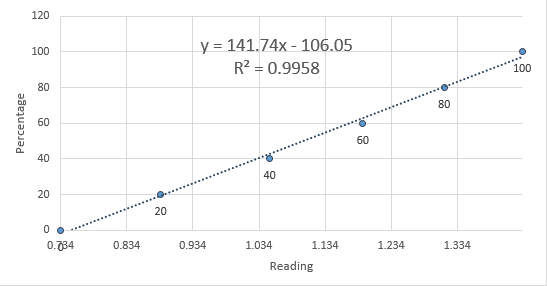
\includegraphics[width=0.4\textwidth]{img_4_5_1}
	\caption{Scatter plot for Table \ref{tab4.5.1}}
	\label{fig:4.5.1}
\end{figure}
Since the equation is given by the software, we can just replace with the reading: $y = 141.74 \times 1.15 - 106.05 \approx 56.951$
\end{solution}

\pagebreak

\section{Exercise 4.5.2}

{\large Consider the following data on the number of hours that 10 persons studied for a French test and their scores:}

\begin{table}[h!]
\centering
\begin{tabular}{@{}cc@{}}
\toprule
Hours studied & Score \\ \midrule
x & y \\
4 & 31 \\
9 & 58 \\
10 & 65 \\
14 & 73 \\
4 & 37 \\
7 & 44 \\
12 & 60 \\
22 & 91 \\
1 & 21 \\
17 & 84 \\ \bottomrule
\end{tabular}
\caption{Hours studied and test scores of 10 individuals}
\label{tab4.5.2}
\end{table}


{\large \textbf{a)} Find the equation of the least squares line that approximates the regression of the test scores on the number of hours studied.}

\begin{solution}
\begin{figure}[h!]
	\centering
	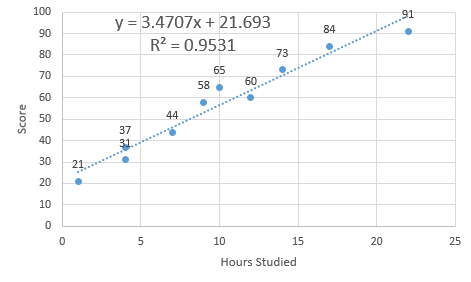
\includegraphics[width=0.4\textwidth]{img_4_5_2}
	\caption{Scatter plot for Table \ref{tab4.5.2}}
	\label{fig:4.5.2}
\end{figure}


This can be obtained \textit{by hand} using the following equation:
\[B = \frac{\sum\limits_{i=1}^n x_i Y_i - \overline{x}\sum\limits_{i=1}^n Y_i}{\sum\limits_{i=1}^n x_i^2 - n \overline{x}^2}\]

Replacing by the required data, we have that $\dfrac{6945 - 5640}{1376 - 1000} = 3.47074$

Now we use the equation $A = \overline{Y} - B\overline{x} = 56.4- 34.70744 = 21.69256$.

Therefore, $Y = 21.69256 + 3.47074x$ is the equation of the line that approximates the regression of the data.

Additionally, a piece of software provides pretty much the same value, as can be seen in Fig. \ref{fig:4.5.2}.
\end{solution}

\spacepls

{\large Predict the average test score of a person who studied 14 hours for the test.}

\begin{solution}
A simple substitution in $Y = 21.69256 + 3.47074x$ yields 70.28292 as the predicted average test score of a person who studied 14 hours for the test.
\end{solution}
\end{document}